\section{Entanglement Properties}
So far, we have thoroughly discussed the density matrices of the Kitaev ground state in various situations. Here, using the density matrices obtained in previous sections, we investigate the structure of the entanglement spectrum of the Kitaev model. 

In this section, we will still represent the final result for the entanglement spectra of the Kitaev model in terms of those of free Majorana fermion systems, as proposed in Ref.~\cite{Yao-Qi}. On the one hand, it is not feasible to directly analyze the entanglement spectra using spin language because of the complex algebraic features of spin operators; On the other hand, the degeneracy in the entanglement spectrum and the block-diagonal feature of the reduced density matrices actually shed more physical insights into the origin of the gauge contribution to the entanglement, as the physical picture provided by Ref.~\cite{PRX-ent-high}. 

\subsection{Entanglement Entropy and its Separability}\label{sec:EE-calculation-even}

In this section, the EE of the Kitaev ground state is calculated using the DM and the algebras of strings obtained earlier, which reproduces the result proposed by~\cite{Yao-Qi_2010} that it can be separated into the gauge and the matter contribution. The derivation reveals that the matter part of the EE reflects the equivalence between representations $\mathcal{S}_\mathfrak{D}$ and $\mathcal{M}_\mathfrak{D}$, while the gauge part arises from the difference in dimension of the Hilbert space between these two identical representations. 



Due to the equivalence of the representations $\mathcal{S}^{(A)}$ and $\mathcal{M}$ in the region $A$, plus the similarity of the forms of Eq.~\eqref{equ.red-DM-new} and \eqref{equ.rho-F-reduced}, the EE of the spin system ${S_A = -\Tr_A\rho_A\ln\rho_A}$ can be calculated using the Majorana DM \eqref{equ.rho-F-reduced} as an alternative. Inspired by this insight, we first observe that both representations $\mathcal{S}^{(A)}$ and $\mathcal{M}$ consist of traceless operators and the identity. Therefore, their trace satisfies 
\begin{equation}\label{equ.U-V-trace-relation}
    \left\{
\begin{aligned}
&\Tr_{A} \mathcal{S}^{(A)}_{\mathfrak{D}} = 2^{N^A-N^A_p}\delta_{\mathfrak{D},\varnothing} \\
& \Tr_{A,F} \mathcal{M}_{\mathfrak{D}} = 2^{N^A/2}\delta_{\mathfrak{D},\varnothing}
\end{aligned}
\right.
\end{equation}
where $\Tr_{A,F}$ stands for taking the trace over the matter sector in the region $A$. For simplicity, we assume the subregion $A$ contains an even number of lattice sites $N^A$. Cases with an odd number of lattice sites will be discussed in later sections. Given that the two representations are identical, the following identity holds for an arbitrary analytic function $f$: 
\begin{equation}\label{equ.identity}
    \Tr_A f(\{\mathcal{S}^{(A)}\}) = \frac{1}{2^{N^A/2 - N^A_p}}\Tr_{A,F} f(\lrg{\mathcal{M}}).
\end{equation}
Given this property, we can define a function
\begin{align*}
    &f(\lrg{\mathcal{R}}) \\
    \equiv& \lrm{\frac{1}{2^{N^A-N^A_p}}\sum_{[\mathfrak{D}]\subset A}\mathfrak{C}_\mathfrak{D}\mathcal{R}_{\mathfrak{D}}}\ln\lrm{\frac{1}{2^{N^A-N^A_p}}\sum_{[\mathfrak{D}]\subset A}\mathfrak{C}_\mathfrak{D}\mathcal{R}_{\mathfrak{D}}},
\end{align*}
where $\mathcal{R}$ stands for an arbitrary representation of the algebra $\anglelr{\lrg{\mathfrak{D}},\ominus}$. With this,{the following two functions that appear in the formula for computing the entropy can be expressed in terms of the function $f$ with different representations as the domain}.
\begin{equation}\label{eq:rholnrho}
    \left\{
    \begin{aligned}
    \rho^F_A\ln\rho_A^F &= \frac{1}{2^{N^A/2-N^A_p}} f\lr{\lrg{\mathcal{M}}}  \\
        &\hspace{3em} - \lrm{\lr{\frac{N^A}{2}-N^A_p}\ln 2}\rho^F_A
        \\
    \rho_A\ln\rho_A &= f(\{\mathcal{S}^{(A)}\})
    \end{aligned}
    \right.
\end{equation}
The EE can be written in terms of the above functions, and the trace over the spin space can be converted to the trace over the matter sector using Eq.~\eqref{equ.identity}
\begin{align*}
    S_A &= -\Tr_A f(\{\mathcal{S}^{(A)}\}) \\
    &= -\frac{1}{2^{N^A/2 - N^A_p}}\Tr_{A,F} f(\lrg{\mathcal{M}}) \\
    &= -\Tr_{A,F} \rho^F_A\ln\rho^F_A + \lr{\frac{N^A}{2}-N^A_p}\ln 2.
\end{align*}
{The last term proportional to $\ln 2$ can be converted to the area-law entanglement.} To demonstrate this, we introduce a geometric relation connecting $N^A$, $N^A_p$, and $\abs{\de A}$ (the proof is given in Appendix~\ref{appendix:Pick}),
\begin{equation}\label{equ.Pick_sim-con}
    \abs{\de A} = N^A - 2N^A_p + 2.
\end{equation}
Due to this relation, the term proportional to $\ln 2$ in the last line of the above derivation can be rewritten in terms of $\abs{\de A}$, 
\begin{equation}\label{equ.EE-separation}
    S_A = \underbrace{-\Tr_{A,F}\lr{\rho_A^F\ln\rho_A^F}}_{\equiv S_A^F} + \underbrace{\lr{\frac{1}{2}\abs{\de A}-1}\ln 2}_{\equiv S_A^G}.
\end{equation}
This formula shows that the EE can be separated into the matter part $S^F_A$ and the gauge part $S^G_A$, in agreement with the result in Ref.~\cite{Yao-Qi_2010}. 
%
{
The decomposition in Eq.~\eqref{equ.EE-separation} has a direct structural interpretation at the level of the physical RDM. 
%
As we demonstrate in the following sections, the matter contribution is encoded in the eigenvalue spectrum within each identical block of the RDM, whereas the gauge contribution originates from the exact multiplicity of these blocks and therefore from the associated degeneracy of the entanglement spectrum.
%
This block organization is enforced by the gauge structure of the physical spin Hilbert space, which becomes explicit through the Gauss-law constraint and the exact 1-form Wilson symmetry introduced in sections following Sec.~\ref{sec:block-diagonal-structure}.   
%
Thus, the gauge--matter separation of the EE is not merely an entropy-level identity, but reflects a more fundamental organization of the physical RDM.
%
Below, we discuss the two contributions separately.
}
%


{
The matter contribution to the EE calculated from Eq.~\eqref{equ.rho-F-reduced} depends on the model details encoded in the spin correlation functions. It can be computed exactly in the Kitaev model because the equivalent Majorana fermion system is free, where all information about the state is encoded in the two-point correlation functions~\cite{Jin-Korepin_2004, Vidal-Latorre-Rico-Kitaev_2003, Latorre-Rico-Vidal_2004, Peschel_2003, Peschel-Eisler_2009, Chung-Peschel_2001, Cheong-Henley_2004}. The single-particle ES is the eigenvalue spectrum of the correlation matrix $\Gamma^{(c)}$, which is of size $N^A\times N^A$, defined as
\begin{equation}
    [\Gamma^{(c)}]_{ij} \equiv \frac{1}{2}\anglelr{c_ic_j}\quad ;\quad i,j\in A.
\end{equation}
The eigenvalues of $\Gamma^{(c)}$, denoted by $\gamma_{k,\pm}$, can be expressed in pairs if $N^A$ is even~\cite{Jin-Korepin_2004, Latorre-Rico-Vidal_2004}
\begin{equation}\label{equ.gamma-eigenvalue}
    \gamma_{k,\pm} = \frac{1 \pm \nu_k}{2} \quad ; \quad k = 1,2,\cdots, \frac{N^A}{2}.
\end{equation}
In this way, the contribution of the matter to EE becomes 
\begin{equation}\label{equ.EE-corr-mat}
    S_A^F = -\tr\lr{\Gamma^{(c)}\ln\Gamma^{(c)}}.
\end{equation}
The trace ``$\tr$'' is written in lowercase here to distinguish it from the trace ``$\Tr$'' over the Hilbert space of the quantum many-body system. This quantity can be computed via numerically diagonalizing the correlation matrix $\Gamma^{(c)}$. In terms of the correlation matrix, Eq.~\eqref{equ.EE-separation} can be written as
\begin{equation}\label{equ.Yao-Qi-standard-form}
    S_A = -\tr\lr{\Gamma^{(c)} \ln \Gamma^{(c)}} + \lr{\frac{1}{2}\abs{\de A} - 1}\ln 2.
\end{equation}

The gauge contribution, by contrast, originates from the mismatch in dimension between the physical spin Hilbert space and the equivalent Majorana-fermion Hilbert space justified by the algebraic equivalence between the spin representation $\mathcal{S}$ and the Majorana representation $\mathcal{M}$ of the Kitaev ground state, as represented by the term proportional to $\ln 2$ appearing in Eq.~\eqref{eq:rholnrho}. This holds independently of specific model details such as coupling constants or lattice geometry. This Hilbert-space dimensional mismatch, combined with the geometric relation~\eqref{equ.Pick_sim-con}, naturally gives rise to the area-law scaling of $S^G_A$. Here, the scaling coefficient $1/2$ indicates that each gauge degree of freedom residing on the edges crossing the entanglement cut contributes only half a bit of entropy, as the other half is accounted for by the fractionalized matter fermions. At this stage, the topological entanglement entropy $-\ln 2$ appearing in $S^G_A$ originates from the geometric relation~\eqref{equ.Pick_sim-con}. We elucidate its physical interpretation and its connection to the boundary-variable parity in sections following Sec.~\ref{sec:block-diagonal-structure}. Unlike the matter contribution $S^F_A$, which depends on model details, the explicit derivation of $S^G_A$ indicates that the gauge contribution to the EE relies on a more fundamental property: namely, the block organization of the physical RDM, as mentioned earlier.
}




\subsection{Interplay between Entanglement and Subsystem Fermion Parity}\label{sec:EE-calculation-odd}

A subtlety arises when the number of lattice sites in a subregion is odd, since a well-defined Hilbert space of a Majorana fermion system must have an even number of Majorana fermions. We address the problem in this section and demonstrate how this even-odd problem, i.e., the \textit{fermion parity}, is intertwined with the entanglement structure. Understanding subsystem fermion parity provides crucial insights into formulating and resolving this ambiguity directly within the physical spin representation.

To resolve the issue of odd $N^A$, we add a redundant Majorana fermion, denoted by $c_{(N^A+1)}$, to the original system, making the number of Majorana fermions even, so that our previous approach works again~\cite{Lee-Wilczek_2013}. We design the redundant Majorana fermion in such a way that it has no interaction with other Majorana fermions. Mathematically, we set $\sanglelr{ c_{(N^A+1)}c_i}=0\;\forall i\in A$. In this way, the dimension of the Hilbert space of the matter sector, including the redundant one, is $2^{(N^A+1)/2}$, and the RDM becomes
\begin{equation}\label{equ.rho-A-F-odd}
    \rho_A^{F} = \frac{1}{2^{\lr{N^A+1}/2}}\sum_{[\mathfrak{D}]\in A}\mathfrak{C}_{\mathfrak{D}}\mathcal{M}_\mathfrak{D}
\end{equation}
The redundant Majorana fermion does not enter the DM. Thus, the form of $\rho^F_A$ remains intact. Only the normalization coefficient is changed. With the redundant Majorana fermion, the original correlation matrix $\Gamma^{(c)}$ is correspondingly enlarged by one dimension to $\Tilde{\Gamma}^{(c)}$. According to the definition of $c_{(N^A+1)}$, we obtain
\begin{equation}\label{equ.tilde-Gamma-corner}
    \Tilde{\Gamma}^{(c)} = 
\lr{
\begin{array}{c|c}
    \Gamma^{(c)} & 0 \\
    \hline
    0 & 1/2
\end{array}
}.
\end{equation}
In the enlarged correlation matrix $\Tilde{\Gamma}^{(c)}$, the upper-left block is the original correlation matrix. The upper-right column and the lower-left row are zeros because the redundant Majorana fermion does not correlate with others. The element $1/2$ at the lower-right entry is given by the redundant Majorana fermion $\frac{1}{2}=\frac{1}{2}\sanglelr{c_{(N^A+1)}c_{(N^A+1)}}$. 

Due to the change in the dimension of the Hilbert space of the matter sector, the relation \eqref{equ.U-V-trace-relation} needs to be modified to the following
\begin{equation}\label{equ.U-V-trace-relation-odd}
    \left\{
\begin{aligned}
&\Tr_{A} \mathcal{S}^{(A)}_{\mathfrak{D}} = 2^{N^A-N^A_p}\delta_{\mathfrak{D},\varnothing} \\
& \Tr_{A,F} \mathcal{M}_{\mathfrak{D}} = 2^{(N^A+1)/2}\delta_{\mathfrak{D},\varnothing}
\end{aligned}
\right..
\end{equation}
Performing the same calculation as we did in the cases with even $N^A$, we obtain a result similar to the EE 
\begin{align}\label{equ.EE-odd-derive-1}
    S_A &= -\Tr_{A,F} \rho^F_A\ln\rho^F_A + \lr{\frac{N^A-1}{2}-N^A_p}\ln 2 \nonumber\\
    &= -\tr\lr{\Tilde{\Gamma}^{(c)}\ln \Tilde{\Gamma}^{(c)}} + \lr{\frac{1}{2}\abs{\de A} - \frac{3}{2}}\ln 2,
\end{align}
where the correlation matrix in Eq.~\eqref{equ.EE-corr-mat} is replaced by the enlarged one. According to Eq.~\eqref{equ.tilde-Gamma-corner}, the first term of Eq.~\eqref{equ.EE-odd-derive-1} can be reduced and expressed in terms of the original correlation matrix 
\begin{equation}\label{equ.EE-reduce}
    \tr\lr{\Tilde{\Gamma}^{(c)} \ln \Tilde{\Gamma}^{(c)}} = \tr\lr{\Gamma^{(c)} \ln \Gamma^{(c)}} - \frac{1}{2}\ln 2 .
\end{equation}
Substituting Eq.~\eqref{equ.EE-reduce} into Eq.~\eqref{equ.EE-odd-derive-1}, the last term $-\frac{1}{2}\ln 2$ in Eq.~\eqref{equ.EE-reduce} will cancel the term $-\frac{1}{2}\ln 2$ in Eq.~\eqref{equ.EE-odd-derive-1} arising from the enlarged dimension of the matter sector, and we ultimately obtain a result that is the same as Eq.~\eqref{equ.Yao-Qi-standard-form} for even $N^A$. 

The above derivation not only confirms that the result in Ref.~\cite{Yao-Qi_2010} remains valid for subsystems with an odd number of sites $N^A$, but also provides a new physical insight into the interplay between the matter and gauge sectors. Operationally, we first borrow a dimension $2^{1/2}$ of a single Majorana fermion from the gauge sector to make the Hilbert space of the matter sector well-defined. The resulting shift of $-\frac{1}{2}\ln 2$ reflects this borrowed dimension. Subsequently, the redundant fermion yields the term $+\frac{1}{2}\ln 2$, effectively restoring the dimension back to the gauge sector and leaving no net change. 

Having established the entropy formula for odd $N^A$, we now examine the ES in this situation and its intimate connection with the subsystem fermion parity. As shown in Eq.~\eqref{equ.gamma-eigenvalue}, the elements in the single-particle ES come in pairs. Since the lower-right corner of Eq.~\eqref{equ.tilde-Gamma-corner} provides an eigenvalue $1/2$, there must be another identical eigenvalue $\frac{1}{2}=1-\frac{1}{2}$ in the original single-particle ES. Therefore, the many-body ES can be written as 
\begin{equation}\label{equ.many-body-entanglement-spectrum-odd}
\lambda_{n_1,n_2,\cdots,n_{(N^A+1)/2}} = \frac{1}{2}\prod_{k=1}^{\frac{N^A-1}{2}}\gamma_{k,n_k}
\end{equation}
The formula shows that the many-body ES depends on only $(N^A-1)/2$ quantum numbers, although the complete labeling contains $(N^A+1)/2$ of them. In other words, there is a twofold degeneracy in the ES of the matter sector. Thus, we only have $2^{\frac{N^A-1}{2}}$ distinct values of $\lambda_{\lrg{n}}$. The degree of degeneracy for each distinct eigenvalue is therefore $2^{\frac{N^A+1}{2}-N^A_p}$ because the total number of eigenvalues is equal to the number of distinct eigenvalues multiplied by the number of degeneracies
\[
2^{N^A-N^A_p} = 2^{\frac{N^A-1}{2}}\times 2^{\frac{N^A+1}{2}-N^A_p}.
\]
Due to the conservation of fermion parity in the subregion $A$, the fermion parity operator, defined by $\hat{\bog{\pi}}^{(A)} = i^{N^{A}}\prod_{j\in A}c_j$, commutes with the RDM. From the fermion-parity point of view, the twofold degeneracy in the matter sector can be understood as a block-diagonalization that depends on the subsystem fermion parity. As we have seen, the value of $\lambda_{\lrg{n}}$ is independent of the last fermion number $n_{(N^A+1)/2}$. At the same time, $\hat{\bog{\pi}}^{(A)}$ commutes with the entanglement Hamiltonian, and hence also commutes with $\rho_A$. Therefore, ES divides into even and odd sectors, and these two identical sectors correspond to $\lrg{n}$ with $n_{(N^A+1)/2}=0,1$, respectively, giving a twofold degeneracy in ES of the matter sector. The microscopic origin of this degeneracy in terms of the physical spin RDM is discussed in Sec.~\ref{sec:origin_degeneracy_odd}.


\subsection{Block-Diagonal Structure of Density Matrices}\label{sec:block-diagonal-structure}
\valert{
The fact that the spin representation $\mathcal{S}$ and the Majorana representation $\mathcal{M}$ are identical implies that the reduced density matrix might be of a block-diagonal form, in which the blocks are all identical. In this section, we discuss those operators that block-diagonalize the density matrix and elucidate their relation with the emergent gauge field. 
%
%However, this is only a hypothesis instead of a direct and rigorous proof of the existence of such a structure. 
%
%To see that the density matrix indeed has such a block-diagonal structure, we have to find the operator corresponding to each block that commutes with the density matrix. They are expected to be related to the emergent gauge fields, given that they give the gauge contribution of the entanglement.

%In addition, to make every block identical, there must be operators that provide equivalence relations among blocks.
}

In light of the physical pictures given by \cite{Yao-Qi_2010} and \cite{Xu-Rakovszky-Knap-Pollmann_2025}, the operators that block-diagonalize the density matrix are defined at the boundary of the subregion because the block-diagonal structure of the reduced density matrix is due to the Gauss law of the gauge field~\cite{Xu-Rakovszky-Knap-Pollmann_2025}. Suppose the Gauss law in a gauge theory defined on a lattice is $\sum_{j\in \mathcal{N}_i}E_{ij} = \rho_i$, where $\rho_i$ is the matter field on the lattice site $i$, $E_{ij}$ is the electric field residing on the edge $\anglelr{ij}$, and $\mathcal{N}_i$ is the set of nearest neighbors of the site $i$. The boundary of the chosen subregion \textit{splits} the Gauss law of some neighborhoods $\mathcal{N}_i$ that cross the boundary, causing entanglement between the subregion and the environment because the Gauss law relates the matter field outside the subregion with the gauge field at the boundary, which is partly inside the subregion. Each \textit{residue} Gauss law at the boundary then acts as a symmetry operator that block-diagonalizes the reduced density matrix. 

In the Kitaev model, a problem is that the Gauss law of the gauge theory, which reads $b^x_ib^y_ib^z_ic_i = \mathds{1}$, only exists in the Majorana representation. Another issue is that the fundamental degrees of freedom of the Kitaev model reside on the lattice sites of the lattice, but the electric field operators $E_{ij}$ of the gauge theory, defined by $\mrm{e}^{i E_{ij}} = b^{\alpha_{ij}}_i$, live on edges, and which are not well-defined in the original setting of the model. For these reasons, we cannot directly apply the method proposed by~\cite{Xu-Rakovszky-Knap-Pollmann_2025}. %Some modifications are necessary.

Our solution to this issue is to transform a Majorana fermion theory coupled to a gauge field back to the physical spin representation by \textit{gluing} pairs of fermions using string operators. 
%As we have noted earlier, the residual electric field inside the subregion after tracing out the environment is proportional to the exponent of $b$-Majorana fermions at the boundary, with the direction pointing outward. 
Suppose there are an even number $\abs{\de A} = 2L$ of edges that cross the boundary of the simply-connected region $A$. The corresponding set of $b$-Majorana fermions encoding the residual electric field is $\lrg{b^{\mu_1}_{i_1}, b^{\mu_2}_{i_2}, b^{\mu_3}_{i_3},\cdots,b^{\mu_{2L}}_{i_{2L}}}$, where $\mu_k$ represents the direction of the $k$-th edge crossing the boundary, which is connected to site $i_k$. 
To transform these $b$-Majorana fermions to a physical representation, we insert gauge-field operators along strings $\mathcal{C}_1, \mathcal{C}_2, \mathcal{C}_3,\cdots, \mathcal{C}_{L}$ that link pairs of Majorana fermions $(b^{\mu_1}_{i_1},b^{\mu_2}_{i_2}), (b^{\mu_3}_{i_3},b^{\mu_4}_{i_4}),\cdots,(b^{\mu_{2L-1}}_{i_{2L-1}},b^{\mu_{2L}}_{i_{2L}})$, respectively, to create a series of physical operators of the form
\begin{equation}\label{equ.b-link}
    b^{\mu_{2n-1}}_{i_{2n-1}} \lr{\prod_{\anglelr{ij}\in\mathcal{C}_{n}} \hat{u}_{ij}}b^{\mu_{2n}}_{i_{2n}} \quad ; \quad n=1,2,3,\cdots, L
\end{equation}
in which the two $b$-Majorana fermions $b^{\mu_{2n-1}}_{i_{2n-1}}$ and $b^{\mu_{2n}}_{i_{2n}}$ are at the endpoints of the string $\mathcal{C}_n$, and the product of gauge-field operators in between is the string that links the two endpoints together. 
\begin{figure}
    \centering
    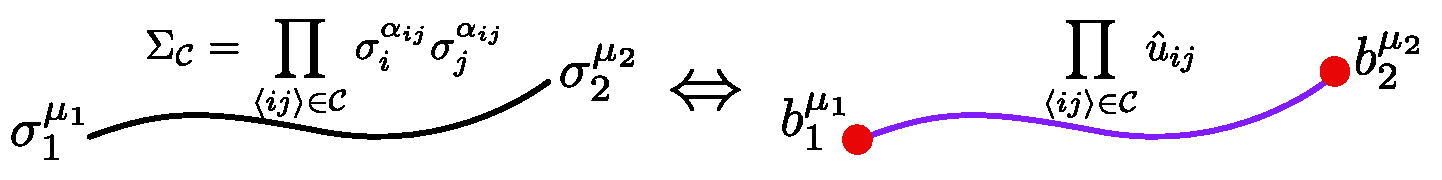
\includegraphics[width=\linewidth]{figures/linking-string-electric-field.pdf}
    \caption{Two $b$-Majorana fermions can also be linked by a series of gauge-field operators, $\prod_{\anglelr{ij}\in\mathcal{C}} \hat{u}_{ij}$. In that way, a physical operator $\hat{\xi}$ is constructed.}
    \label{fig.linking-strings-electric-field}
\end{figure}
However, the expression \eqref{equ.b-link} only contains $b$-Majorana fermions and cannot be transformed directly to the spin representation. To obtain physical strings containing purely spin operators, we can further insert $c$-Majorana fermions into the expression \eqref{equ.b-link}, then we obtain the following result   
\begin{equation}\label{equ.c-b-link}
    b^{\mu_{2n-1}}_{i_{2n-1}}c_{i_{2n-1}} \lr{\prod_{\anglelr{ij}\in\mathcal{C}_{n}} c_i\hat{u}_{ij}c_j}c_{i_{2n}}b^{\mu_{2n}}_{i_{2n}}.
\end{equation}
%in which those inserted $c$-Majorana fermions are identities $cc=\mathds{1}$, thus everything remains the same. 
%
After considering the transformation $\sigma^\mu_i\to ib^\mu_ic_i$, the operator \eqref{equ.c-b-link} is equal to the operators $\hat{\xi}_n$ defined in the following way
\begin{equation}\label{equ.spin-string-linking-gauge}
    \hat{\xi}_n \equiv \sigma^{\mu_{2n-1}}_{i_{2n-1}}\Sigma_{\mathcal{C}_n}\sigma^{\mu_{2n}}_{i_{2n}} \quad ; \quad n=1,2,3,\cdots ,L
\end{equation}
up to a phase that depends on the lengths of the strings $\abs{\mathcal{C}_n}$. The process of producing $\hat{\xi}$-operators from \eqref{equ.b-link} to \eqref{equ.spin-string-linking-gauge} is illustrated in \autoref{fig.linking-strings-electric-field}. All $\hat{\xi}_n$ operators defined in a simply-connected subregion $A$ commute with the reduced density matrix $\rho_A$. 
\begin{figure}
    \centering
    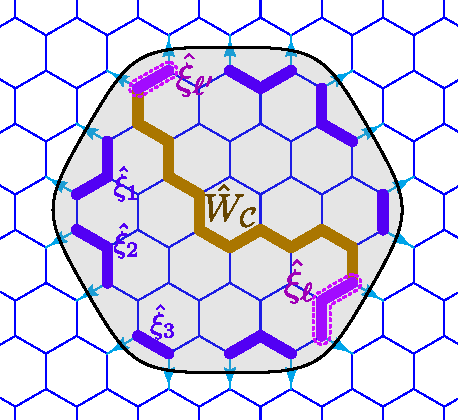
\includegraphics[width=0.8\linewidth]{figures/xi-wilson-flip.pdf}
    \caption{\alert{The electric-field operators living on the edges crossing the boundary of the region are split in half, as shown in the first panel. In the physical spin representation, these electric fields correspond to the spin operators $\sigma^\mu$ with directions pointing outwards. The second panel displays string operators that connect two adjacent spins in the first panel in a pair. Multiplying the first panel by the second one gives a series of operators $\hat{\xi}$, as shown in the third panel. Applying the same method but with the pairing order shifted yields another set of operators $\hat{\zeta}$, as showcased in the last panel.}}
    \label{fig.xi-def}
\end{figure}
The first three panels of \autoref{fig.xi-def} illustrate an example of the process of defining $\hat{\xi}$-operators using the method given by \eqref{equ.spin-string-linking-gauge}. 
%The directions of the spin operators at the endpoints of the links point outward, representing the gauge fields being cut. In the first panel are the spin operators $\sigma^\mu_i$, which are exactly the spin operators shown in equation \eqref{equ.spin-string-linking-gauge}, at the boundary with their directions pointing outwards. In the next panel, we subsequently multiply the string operators $\Sigma_{\mathcal{C}_n}$, which is the string operator shown in equation \eqref{equ.spin-string-linking-gauge} that lies between the two spin operators residing on the two endpoints of the string, with the spin operators set previously. After that, such operators are used as definitions of $\hat{\xi}_n$'s, which are illustrated in the third panel of \autoref{fig.xi-def}. In this example, we now focus on $\hat{\xi}_1$, which is defined as
%\[
%\hat{\xi}_1 = \sigma^y_1\lr{\sigma^x_1\sigma^x_2}\sigma^z_2 \propto \sigma_1^z\sigma_2^y.
%\]
%The subscript ``1'' indicates the lower-left endpoint of the dimer, while ``2'' stands for the other one. It can be shown that $\hat{\xi}_1$ commutes with every string operator $\Sigma_{\mathfrak{D}}$ with $\mathfrak{D}\subset A$ in a trivial way by examining all possible strings that reach the two endpoints of the dimer where $\hat{\xi}$ lives. By doing so, one will find that either (i) at one endpoint of a string $\mathcal{C}$, which is right at one of the two endpoints of the $\hat{\xi}_1$ dimer, is a spin operator whose direction is parallel to the spin operator of $\hat{\xi}_1$ on that endpoint; Or (ii) none of the two spin operators of $\Sigma_{\mathcal{C}}$, whose positions are the two endpoints of $\hat{\xi}_1$, is parallel to the spin operator of $\hat{\xi}_1$ at its position, such that the twice of sign flipping caused by the anti-commutation of Pauli algebra between $\Sigma_{\mathcal{C}}$ and $\hat{\xi}_1$ gets the positive sign again. 
%These situations, along with the fact that $[\hat{\xi}_1,W_p]=0\;\forall p$~\footnote{A loop also counts as a string, just with two endpoints at the same position, therefore, proving that every string operator commutes with $\hat{\xi}_n$ also proves that every plaquette operator commutes with $\hat{\xi}_n$ at the same time.}, 
By exhausting all possible string operators in the subregion and the commutation relations among spin operators, we prove that $[\hat{\xi}_n,\rho_A]=0\;\forall n$ because $\rho_A$ consists of string operators inside $A$. 
%In the same sense, we may generalize this statement to $[\hat{\xi}_n,\rho_A]=0\;\forall n$, where the operators $\hat{\xi}_n$ are defined through the process illustrated in \autoref{fig.xi-def} in $A$. 
At the same time, the regions where $\hat{\xi}$-operators are supported have no intersection, hence they commute with each other, $[\hat{\xi}_m,\hat{\xi}_n]=0\;\forall m,n$. Therefore, the set $\lrg{\xi_1,\cdots,\xi_L}$ of expectation values of $\hat{\xi}$-operators defined in $A$ forms good quantum numbers that block-diagonalizes the reduced density matrix $\rho_A$
\begin{equation}\label{equ.rho-block-diagonal-structure}
    \rho_A = \bigoplus_{\lrg{\xi_1,\cdots,\xi_L}} \varrho_{\lrg{\xi_1,\cdots,\xi_L}}
\end{equation}
where each $\varrho_{\lrg{\xi}}$ is the block labeled by a set of binaries $\lrg{\xi}$, and thus the number of blocks is $2^{L} = 2^{\abs{\de A}/2}$.

\alert{In defining $\hat{\xi}$-operators, the way we chose to pair points along the boundary was like $(b^{\mu_1}_{i_1},b^{\mu_2}_{i_2}), (b^{\mu_3}_{i_3},b^{\mu_4}_{i_4}),\cdots,(b^{\mu_{2L-1}}_{i_{2L-1}},b^{\mu_{2L}}_{i_{2L}})$. However, it is not the only way to pair these points. We can choose another way in which the pairing order is shifted by one compared to the previous way we adapted for $\hat{\xi}$-operators
\[
(b^{\mu_2}_{i_2},b^{\mu_3}_{i_3}), (b^{\mu_4}_{i_4},b^{\mu_5}_{i_5}),\cdots,(b^{\mu_{2L}}_{i_{2L}},b^{\mu_1}_{i_1})
\]
and then connect each of them through a new set of strings $\{\mathcal{C}'_n\}$. In this way, a set of operators $\hat{\zeta}_n$ can be defined
\begin{equation}\label{equ.spin-string-linking-gauge-zeta}
    \hat{\zeta}_n \equiv \sigma^{\mu_{2n}}_{i_{2n}}\Sigma_{\mathcal{C}'_n}\sigma^{\mu_{2n+1}}_{i_{2n+1}} \quad ; \quad n=1,2,3,\cdots, L
\end{equation}
where the periodic notational convention $i_{2L+1}=i_1$ and $\mu_{2L+1}=\mu_1$ is used. In the same sense, these $\hat{\zeta}$-operators also commute with the reduced density matrix. An example of a set of $\hat{\zeta}$-operators is illustrated in the fourth panel of \autoref{fig.xi-def}, from which we can see that the pattern of $\hat{\zeta}$-operators differs from that of $\hat{\xi}$-operators by shifting a unit along the boundary, so that each $\hat{\xi}_n$ is in between $\hat{\zeta}_{n-1}$ and $\hat{\zeta}_n$. According to the algebraic rules of Pauli matrices, a relation between $\hat{\xi}$-operators and $\hat{\zeta}$-operators can be obtained directly
\begin{equation}\label{equ.xi-zeta-relation}
    \hat{\zeta}_n\hat{\xi}_m\hat{\zeta}_{n} =
\left\{
\begin{array}{ll}
   -\hat{\xi}_m &;\; \text{for $m=n\vee n+1$} \\
   \hat{\xi}_m  &;\; \text{otherwise} 
\end{array}
\right.
\end{equation}
This equation implies that the $\hat{\zeta}$-operators relate different blocks of the density matrix $\rho_A$ in the way that
\begin{equation}\label{equ.related-blocks}
    \hat{\zeta}_n \varrho_{\lrg{\cdots,\xi_n,\xi_{n+1},\cdots}}\hat{\zeta}_n^\dagger = \varrho_{\lrg{\cdots,-\xi_n,-\xi_{n+1},\cdots}}
\end{equation}
By this relation, any two blocks $\varrho_{\lrg{\xi}}$ and $\varrho_{\lrg{\xi'}}$ in $\rho_A$ can be related, and thus their sets of eigenvalues are identical. However, a $\hat{\zeta}$-operator flips the eigenvalues of two $\hat{\xi}$-operators at the same time, so only two blocks with the same total parity $\prod_{i=1}^{L}\xi_i$ of the set $\lrg{\xi}$ are related by a specific set of $\hat{\zeta}$-operators.}




\subsection{Origin of Degeneracy}\label{sec:origin_of_degeneracy}

\valert{
The block-diagonal structure of $\rho_A$ implies a massive degeneracy in the entanglement spectrum, since all the blocks in the density matrix are identical. In this section, we interpret a direct correspondence between the gauge part of the entanglement and the degeneracy in the entanglement spectrum. We also explain the emergence of the matter part of the entanglement.
}

Based on the block-diagonal structure \eqref{equ.rho-block-diagonal-structure} of $\rho_A$ and the fact that $\zeta$-operators can relate different blocks, explained by \eqref{equ.related-blocks}, we then conclude that there are 
\[2^{L-1} = 2^{\abs{\de A}/2 - 1}\] 
identical blocks in $\rho_A$. The reason why we only have the number $2^{L-1}$ instead of $2^L$, which is the number of blocks in \eqref{equ.rho-block-diagonal-structure}, is that $\zeta$-operators can only relate blocks with the same parity of the set of quantum numbers $\lrg{\xi}$, so the number of blocks, $2^L$, is actually twice the number of identical blocks. The factor $2^{-1}$ arising from the fixed parity of quantum numbers can also be understood as originating from the exact 1-form Wilson symmetry~\cite{PRX-ent-high}, which is $[\Tilde{W}_h,H] = [\Tilde{W}_v,H] = [W_p,H]=0\;\forall p$. After tracing out the environment $\overline{A}$, the global Wilson operator in the sense of merely the subregion $A$ becomes a string with two endpoints attached to the boundary of $A$, and commutes with $\rho_A$ at the same time. The two endpoints of the Wilson operator can flip the residual $\mathbb{Z}_2$ gauge field at the boundary, playing a role in relating different blocks of $\rho_A$. This is completely the same as the $\zeta$-operators. Based on the block-diagonal structure of $\rho_A$, it can be expressed as
\begin{equation}\label{equ.block-rho-final}
    \rho_A = \bigoplus_{n=1}^{2^{L-1}}\varrho^{(n)}_A
\end{equation}
with all the blocks $\varrho_A^{(n)}$ identical. Substitution of such an expression into the definition of von Neumann entropy directly gives the entanglement entropy, 
\begin{align}\label{equ.EE-from-blocks}
    S_A 
    &= -\Tr_A\rho_A\ln\rho_A \nonumber \\
    &= -\Tr_A\lrm{\bigoplus_{n=1}^{2^{L-1}}\lr{\varrho^{(n)}_A \ln \varrho^{(n)}_A}} \nonumber \\
    &= -2^{L-1}\Tr_A\varrho_A \ln \varrho_A \nonumber \\
    &= -\Tr_A\Tilde{\rho}_A\ln\Tilde{\rho}_A + \lr{\frac{1}{2}\abs{\de A} -  1}\ln 2
\end{align}
where $\Tilde{\rho}_A \equiv 2^{L-1}\varrho_A$ is the normalized density matrix
defined to make $\Tr_A\Tilde{\rho}_A=1$. By comparing Eq.~\eqref{equ.EE-from-blocks} with Eq.~\eqref{equ.EE-separation}, we find that each block $\Tilde{\rho}_A$ corresponds to the Majorana reduced density matrix $\rho_A^F$. At the same time, the gauge part $S^G_A$ can be understood as a measure of the number of identical blocks in $\rho_A$, which is exactly the degree of degeneracy in the entanglement spectrum. This agrees with the gauge nature of such a contribution since the degeneracy arises from the block-diagonal structure of $\rho_A$ along with the fact that every block is identical, and the presence of block-diagonal structure is due to the residual electric field from the Gauss law after the environment is traced out. Finally, the topological entanglement entropy $-\ln 2$ is a consequence of the constraint that the total parity of the quantum numbers, $\prod_{n=1}^L\xi_n$, is fixed, and its origin lies in the existence of the 1-form Wilson symmetry, which satisfies our earlier understanding about the topological entanglement entropy. The most important thing is that the full entanglement spectrum of the Kitaev ground state is obtained. Since an entanglement spectrum is defined as the spectrum of a reduced density matrix, formula \eqref{equ.block-rho-final} directly answers that the entanglement spectrum is the eigenvalue spectrum of $\varrho_A$ with $2^{\abs{\de A}/2-1}$-fold degeneracy. As shown by the comparison between \eqref{equ.EE-from-blocks} and \eqref{equ.EE-separation}, we know that the block $\varrho_A$ is proportional to the Majorana fermion density matrix $\rho^F_A$, and whose spectrum can be solved exactly using the method proposed in Ref.~\cite{Jin-Korepin, Vidal-Latorre-Rico-Kitaev, Latorre-Rico-Vidal, Peschel_2003, Peschel_2009, Chung_2001, Cheong_2004}.

From a more fundamental point of view, the set of $\xi$-operators block-diagonalizes every string operator in a way identical to what we have for $\rho_A$ because each of them commutes with every string operator, and hence so is $\mathcal{S}^{(A)}_{\mathfrak{D}}$
\[
[\xi_i,\mathcal{S}^{(A)}_{\mathfrak{D}}]=0 \;\forall i\in\lrg{1,2,\cdots,L}
\]
Similar to equation \eqref{equ.block-rho-final}, every $\mathcal{S}$-operator can also be block-diagonalized as
\begin{equation}\label{equ.U-V-block-relation}
    \mathcal{S}^{(A)}_{\mathfrak{D}} = \bigoplus_{n=1}^{2^{L-1}}\mathcal{M}^{(n)}_{\mathfrak{D}}
\end{equation}
where $\{\mathcal{M}^{(n)}_\mathfrak{D}\}$ is a set of identical blocks of $\mathcal{S}^{(A)}_{\mathfrak{D}}$. To ensure that expression \eqref{equ.U-V-block-relation} satisfies rule \eqref{equ.U-rep-algebra}, we also have to implement such an algebraic rule on every block $\mathcal{M}^{(n)}_{\mathfrak{D}}$, 
\[
\mathcal{M}^{(n)}_{\mathfrak{D}}\mathcal{M}^{(n)}_{\mathfrak{D}'} = \varphi(\mathfrak{D},\mathfrak{D}')\mathcal{M}^{(n)}_{\mathfrak{D}\ominus\mathfrak{D}'}
\]
This is reminiscent of \eqref{equ.V-rep-algebra}, which shows that the $\mathcal{M}$-representation is identical to $\mathcal{S}$. Based on this, we then state that those blocks $\mathcal{M}^{(n)}_{\mathfrak{D}}$ in \eqref{equ.U-V-block-relation} are nothing but $\mathcal{M}$-operators defined in \eqref{equ.V-rep-def}. In short, the gauge-field degree of freedom is actually the number of identical blocks of string operators represented by spins, and each identical block depicts the physics of free Majorana fermions. This precisely reflects the fractionalization of the spin degree of freedom into gauge-field and matter sectors, with the matter sector further fractionalizing into deconfined Majorana fermions.
\subsection{Interplay between Degeneracy and Fermion Parity}\label{sec:origin_degeneracy_odd}

\begin{figure*}
    \centering
    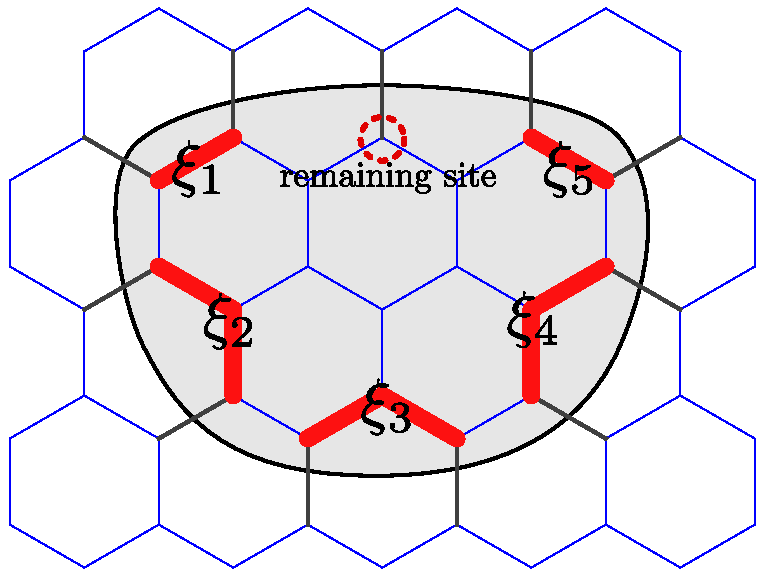
\includegraphics[width=0.25\linewidth]{figures/reshuffle-xi-def-odd.pdf}\hspace{0.5cm}
    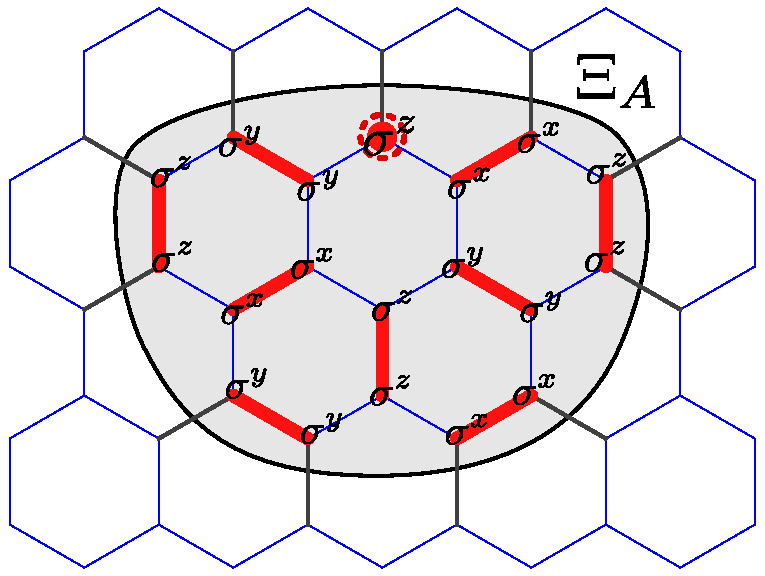
\includegraphics[width=0.25\linewidth]{figures/reshuffle-capital-Xi-def.pdf}\hspace{0.5cm}
    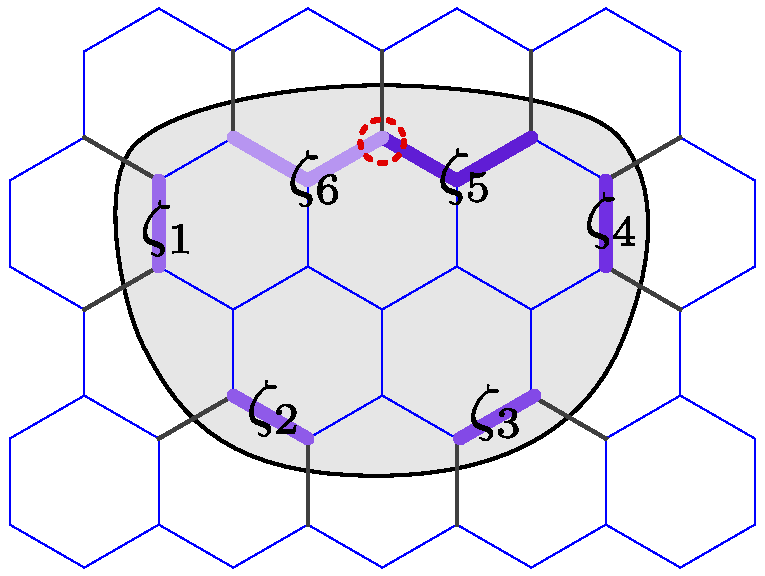
\includegraphics[width=0.25\linewidth]{figures/reshuffle-zeta-def-odd.pdf}
    \caption{For cases with odd $N^A$, there must be a single site $l$ on the boundary that remains unpaired after defining $\hat{\xi}$-operators by pairing the adjacent edges crossing the boundary, as illustrated in the left-most panel. Based on this phenomenon, we can define an operator $\hat{\Xi}_A$ in such a way that the remaining site $l$ is filled in with a Pauli matrix $\sigma^\mu_l$, where $\mu$ is the direction of the edge crossing the boundary that connects to $l$. At the same time, the rest of the part is covered by a dimer covering, as illustrated in the middle panel. On the other hand, the $\hat{\zeta}$-operators are defined in a way similar to what we have introduced, but there are two connected $\hat{\zeta}$-operators sharing one site, which is exactly $l$ after the pairing we have done to define $\hat{\xi}$-operators. In the example illustrated in the right-most panel, the two connected $\hat{\zeta}$-operators are $\hat{\zeta}_5$ and $\hat{\zeta}_6$, and we have $\hat{\zeta}_5\hat{\Xi}\hat{\zeta}_5 = \hat{\zeta}_6\hat{\Xi}_A\hat{\zeta}_6 = -\hat{\Xi}_A$.}
    \label{fig.Xi-odd}
\end{figure*}

\valert{
The notion of fermion parity obtained in Sec.~\ref{sec:EE-calculation-odd} motivates a question: how to describe fermion parity in the spin representation? And how does it give an additional degeneracy in the entanglement spectrum? In this section, we find a specific sort of operator in spin representation that corresponds to fermion parity. It further block-diagonalizes the density matrix if $N^A$ is odd, hence gives an additional degeneracy.
}

A relation implied by equation \eqref{equ.Pick_sim-con} 
\[%\label{equ.bulk-boundary-parity}
    N^A=\abs{\de A} \mod{2},
\]
indicates that once the number of lattice sites in $A$ is odd, so is the length of the boundary. This raises an issue that there will always be one single site left after sorting lattice sites along the boundary in pairs, as shown in the first panel of \autoref{fig.Xi-odd}. If $L$ is defined as the number of $\hat{\xi}$-operators, then in cases with odd $\abs{\de A}$, we onlyl have
\[
L = \frac{1}{2}\lr{\abs{\de A} - 1}
\]
In this way, the block-diagonal structure \eqref{equ.block-rho-final} and the derivation \eqref{equ.EE-from-blocks} are still valid, but the result should be modified as
\begin{align}\label{equ.EE-odd-blocks}
    S_A &= -\Tr_A\Tilde{\rho}_A\ln\Tilde{\rho}_A + \lr{L-1}\ln 2 \nonumber\\
    &= -\Tr_A\Tilde{\rho}_A\ln\Tilde{\rho}_A + \lr{\frac{1}{2}\abs{\de A}-\frac{3}{2}}\ln 2
\end{align}
where $\Tilde{\rho}_A\equiv 2^{L-1}\varrho_A$. The form of \eqref{equ.EE-odd-blocks} is the same as that of \eqref{equ.EE-odd-derive-1}, showing that the block $\Tilde{\rho}_A$ here is identical to the Majorana reduced density matrix \eqref{equ.rho-A-F-odd} with a redundant Majorana fermion included. 

In Sec.~\ref{sec:EE-calculation-odd}, the result of the Majorana entanglement spectrum shows that the degree of degeneracy is 
\[
2^{\frac{N^A+1}{2}-N^A_p} = 2^{\frac{1}{2}\lr{\abs{\de A} - 1}} = 2^L
\]
However, according to the discussion in the previous part for cases with an even number of sites, the degree of degeneracy is $2^{L-1}$ if there are $L$ well-defined $\hat{\xi}$-operators. This discrepancy implies that apart from the set of $\hat{\xi}$-operators, there exists an additional operator that further block-diagonalizes $\rho_A$ to give an additional 2-fold degeneracy to the entanglement spectrum. At the end of Sec.~\ref{sec:EE-calculation-odd}, we have elucidated that the additional 2-fold degeneracy in the entanglement spectrum of the Majorana sector originates from the total fermion parity. Therefore, we anticipate that the additional operator block-diagonalizing the density matrix, which will be denoted by $\hat{\Xi}_A$ later, should be related to the total fermion parity in the Majorana representation. A feasible choice is a dimer covering of the subregion $A$,
\begin{equation}\label{equ.Xi-def}
    \hat{\Xi}_A \equiv \sigma^\mu_l \Sigma_{\mathfrak{D}_{\mrm{DC}}^{A(l)}},
\end{equation}
where the edge configuration $\mathfrak{D}_{\mrm{DC}}^{A(l)}$ stands for a dimer covering of $A$ with a site $l$ being excluded. Since $N^A$ is an odd number, it is not possible for a dimer configuration composed of non-overlapping dimers to cover the entire subregion~\footnote{The dimer covering is not uniquely defined. One can choose an arbitrary dimer covering with a remaining site $l$ at the boundary that covers the subregion.}. The remaining site $l$ is required to be at the boundary of the subregion $A$, and the direction $\mu$ of the Pauli matrix $\sigma_l^\mu$ is that of the edge connected to $l$ that crosses the boundary. An example is illustrated in \autoref{fig.Xi-odd}, where the remaining site $l$ is in the upper portion of the subregion. 

$\hat{\Xi}_A$ can be examined to commute with $\rho_A$ in the same way as used for $\hat{\xi}$-operators. String operators are composed of multiple dimers, and every dimer commutes with the dimer covering because of the properties of Pauli matrices. Therefore, the only thing to be concerned about is $\sigma^\mu_l$ lying at the remaining site.
As we have defined, the site $l$ is at the boundary and $\mu$ points outward. It can be seen directly that, inside $A$, there are only two edges connected to $l$, and the corresponding string operator of both edges anti-commutes with $\sigma^\mu_l$. However, since the string operator also anti-commutes with the dimer that connects to the other endpoint of the edge, the two anti-commutations cancel each other. In the end, every string operator with $\mathfrak{D}\subset A$ commutes with $\hat{\Xi}_A$. Because $\rho_A$ is composed of string operators inside $A$, we conclude that $[\hat{\Xi}_A,\rho_A]=0$. 

$\hat{\Xi}_A$ is related to the total fermion parity by transforming \eqref{equ.Xi-def} into the Majorana fermion representation, and we find that it is equal to the total fermion parity operator multiplied by the gauge-field operators arranged in order of the dimer covering $\mathfrak{D}^{A(l)}_{\mrm{DC}}$
\[
\hat{\Xi}_A \propto \lr{\prod_{\anglelr{ij}\in  \mathfrak{D}^{A(l)}_{\mrm{DC}}} \hat{u}_{ij}} \lr{b^\mu_l\prod_{i\in A}c_i}
\]
up to a phase. In the above formula, the total fermion parity operator is defined as
\begin{equation}\label{equ.total-fermion-parity-odd}
    \hat{\bog{\pi}}^{(A)} \propto b^\mu_l\prod_{i\in A}c_i
\end{equation}
with a phase correction depending on the geometry of the subregion. Because the gauge has been fixed as $u_{ij}=1\;\forall\anglelr{ij}$, the expectation value of $\hat{\Xi}_A$ is completely determined by that of $\hat{\bog{\pi}}^{(A)}$. The definition of the total fermion parity here is different from what we encountered in \eqref{equ.total-fermion-parity-entire-system} and \eqref{equ.total-fermion-parity-Sigma-Z}. In fact, because $N^A$ is an odd number, $\prod_{i\in A}c_i$ itself only contains an odd number of Majorana fermions, hence not sufficient to define a fermion parity operator. This mechanism has been discussed in Sec.~\ref{sec:EE-calculation-odd}, and the alternative we adopted there is to include a redundant Majorana fermion $c_{(N^A+1)}$, and Eq.~\eqref{equ.total-fermion-parity-odd} implies that the redundant fermion is actually $b^\mu_l$ borrowed from the gauge sector. 
%The situation in which the matter sector borrows a Majorana fermion from the gauge sector is also demonstrated in the derivation procedures \eqref{equ.EE-odd-derive-1} and \eqref{equ.EE-reduce}. 
%By now, the physical meaning of the redundant fermion and its origin are clearly reflected by $\hat{\Xi}_A$. 

So far, we have $L$ distinct $\hat{\xi}$-operators and $\hat{\Xi}_A$ that commute with $\rho_A$. These operators give $2^{L+1}$ blocks labeled with a set of eigenvalues $\lrg{\xi_1,\cdots,\xi_L;\Xi_A}$. To prove that these blocks are identical, leading to extensive degeneracy, we also have to find $(L+1)$ $\hat{\zeta}$-operators that relate all the blocks in the same way as \eqref{equ.xi-zeta-relation}. Since $\hat{\zeta}$-operators do not have to commute with each other, we can still find $(L+1)$ of them, as illustrated in the last panel of \autoref{fig.Xi-odd}. The arrangement of $\hat{\zeta}$-operators is designed in a way that two of them overlap at the remaining site $l$. In this way, the $\hat{\xi}$-operators can still be flipped through \eqref{equ.xi-zeta-relation}. More importantly, both overlapping $\hat{\zeta}$-operators can flip the sign of $\Xi_A$. 
%Take \autoref{fig.Xi-odd} for example, these two overlapping operators are $\hat{\zeta}_5$ and $\hat{\zeta}_6$, by which $\hat{\Xi}_A$ can be flipped in the way that $\hat{\zeta}_5\hat{\Xi}_A\hat{\zeta}_5 = \hat{\zeta}_6\hat{\Xi}_A\hat{\zeta}_6 = -\hat{\Xi}_A$. 
%Similar to what we encountered in cases with even $N^A$, 
Since each $\hat{\zeta}$-operator simultaneously flips two values in the set $\lrg{\xi_1,\cdots,\xi_L;\Xi_A}$, they only provide $2^L$-fold degeneracy in the entanglement spectrum although we have $(L+1)$ operators to block-diagonalize $\rho_A$. This agrees with our analysis in Sec.~\ref{sec:EE-calculation-odd}, and the operator $\hat{\Xi}_A$ indeed gives a 2-fold degeneracy to the entanglement spectrum. 

\begin{figure}
    \centering
    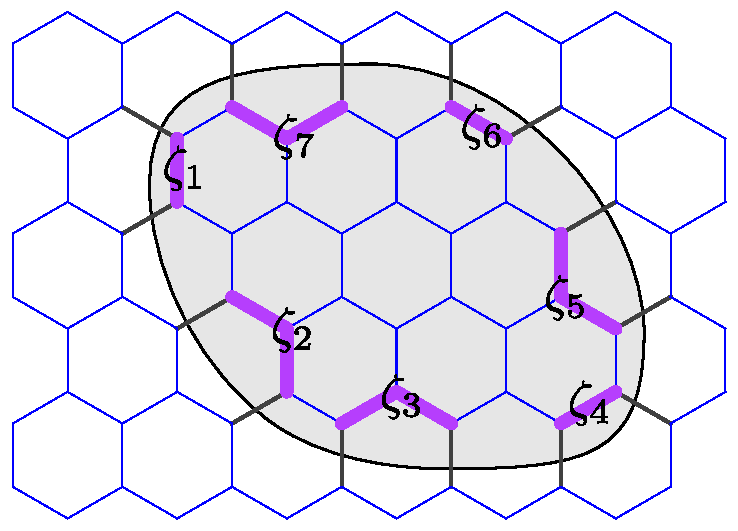
\includegraphics[width=0.4\linewidth]{figures/reshuffle-larger-zeta.pdf}\hspace{0.5cm}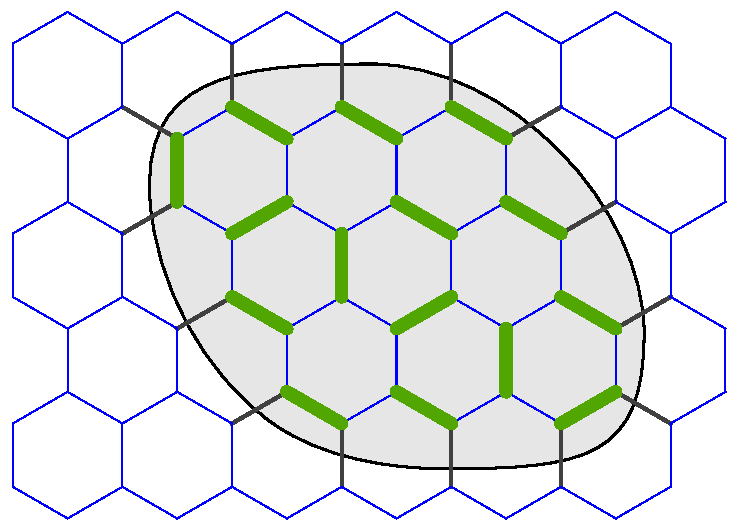
\includegraphics[width=0.4\linewidth]{figures/reshuffle-larger-dimer-covering.pdf}
    \caption{For regions with an even number of lattice sites, at least a dimer covering is well defined, like the one illustrated in the right panel. Assigning a string operator to each dimer in the configuration gives a dimer-covering string operator $\hat{\Xi}_A$ without a single unpaired site, unlike we encountered in cases with an odd number of sites. However, it can be directly checked that $\hat{\Xi}_A$ in this case commutes with every $\hat{\zeta}$-operator. Therefore, such an operator doesn't provide additional degeneracy in the entanglement spectrum.}
    \label{fig.dimer-covering}
\end{figure}
Although it seems that $\hat{\Xi}_A$ can also be defined in cases with even $N^A$ and leads to an additional 2-fold degeneracy, the operator $\hat{\Xi}_A$ defined in this way commutes with every $\hat{\zeta}$-operator, implying that no operator can relate blocks with $\Xi_A=+1$ and $\Xi_A=-1$. As illustrated in \autoref{fig.dimer-covering}, the pattern is simply a dimer covering without a remaining site.  Thus, $\hat{\Xi}_A$ cannot yield a 2-fold degeneracy in the entanglement spectrum in cases with even $N^A$. This constitutes an intrinsic difference between cases with even and odd $N^A$, which is reflected in the total fermion parity in the subregion in the Majorana representation, or equivalently in the dimer covering operator $\hat{\Xi}_A$ in the physical spin formulation.


